% !TeX spellcheck = en_US
\addscenariosection{1}{Cooperative Scenario}{Stand United}{\images/interference.png}

\begin{multicols}{2}

\textbf{Author:} NeuroN

\textbf{Source:} \href{https://discord.com/channels/740870068178649108/1332731339614453802/1332731339614453802}{Archon Studio Discord}

\textit{Evil Dragon Lords threaten entire Enroth. Heroes, with their armies united, march against them in an epic final stand.}

\subsection*{\MakeUppercase{Scenario Length}}

This Scenario is played over 9 Rounds.

\subsection*{\MakeUppercase{Player Setup}}

\textbf{Player Count:} 2--4

\textbf{Starting Resources:} 6 \svg{gold}, 2 \svg{building_materials}, 1 \svg{valuables}

\textbf{Starting Income:} 10 \svg{gold}, 0 \svg{building_materials}, 0 \svg{valuables}

\textbf{Starting Units:}
\begin{itemize}
  \item  1 × A Few cheapest \svgunit{bronze} Units
  \item  1 × A Few cheapest \svgunit{silver} Units
\end{itemize}

\textbf{Town Buildings:} \svgunit{bronze} Dwelling

\subsection*{\MakeUppercase{Map Setup}}

Take the following Map Tiles and arrange them as shown in the Scenario map layout ($P$ stands for the number of players):

\begin{itemize}
  \item P × Starting (I) Map Tile
  \item P × Far (II--III) Map Tile
  \item P × Near (IV--V) Map Tile, all of which must contain an Obelisk
  \item 1 × Center (VI--VII) Map Tile which must contain a Dragon Utopia
\end{itemize}

\subsection*{\MakeUppercase{AI Enemy Setup}}

\textbf{Enemy Deck:} 6 × Might Card, 4 × Magic Card, 4 × Skill Card

\textbf{Enemy Spells:} 1 × Fireball, 1 × Lightning Bolt, 1 × Weakness, 1 × Curse

\textbf{Enemy Skill:} Sorcery

\subsection*{\MakeUppercase{Victory Conditions}}

After every player won a fight in the Dragon Utopia, all players win the Scenario.

\subsection*{\MakeUppercase{Defeat Conditions}}

At least one player failed to beat Dragon Utopia by the end of Round 9.

\subsection*{\MakeUppercase{Timed Events}}
\textbf{\nth{4} Round:}
\begin{itemize}
  \item Roll a \svg{resource} and resolve the result.
\end{itemize}
\textbf{\nth{6} Round:}
\begin{itemize}
  \item Repeat the event of Round 4.
\end{itemize}
\textbf{\nth{8} Round:}
\begin{itemize}
  \item Repeat the event of Round 4.
\end{itemize}

\subsection*{\MakeUppercase{Additional Rules}}

\begin{itemize}
  \item Remove both Azure Dragons Cards from the neutral Units Deck, set one of them aside for later use.
  \item Players cannot recruit secondary Heroes.
  \item Level VII combat cannot be skipped by diplomacy, or any other means.
  \item Players can use their 🔨Build Token to initiate trade with one other chosen player. The two players can freely exchange resources and can exchange artifacts or spells from their hand as if their Heroes were adjacent.
  \item During a game players assemble a shared army. Every player can field Units from the shared army during combat (Shared Units' \svg{map} Map abilities can be activated each Round by only one player).
  \item Upon flagging an Obelisk, discard the top Card from each neutral unit Deck except azure. You can recruit one of these Units. Units bought this way go into shared army.
  \item When fighting on Dragon Utopia one of the neutral Azure Units is always Azure Dragons and the neutral army uses the AI Card Deck. Reshuffle AI Deck and AI Spell Deck at the end of combat.
  \item After winning a fight at Dragon Utopia, no Cube is placed on the dragon utopia. The Victorious Player puts one of their surviving faction Units into the shared army and can redistribute their remaining resources among other players, after which that Player gets removed from the game.
\end{itemize}

\columnbreak

\begin{center}
  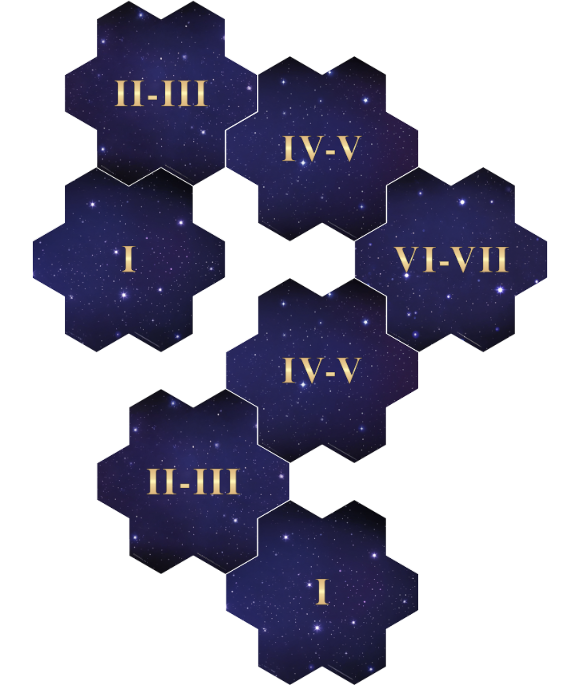
\includegraphics[width=0.7\linewidth]{\maps/stand_united_2p.png}
  \captionof{figure}{\footnotesize\textbf{2-PLAYER SCENARIO}}
\end{center}

\vspace*{\fill}

\end{multicols}

\begin{tikzpicture}[overlay]
  \centering
  \node at (14.1, 0) {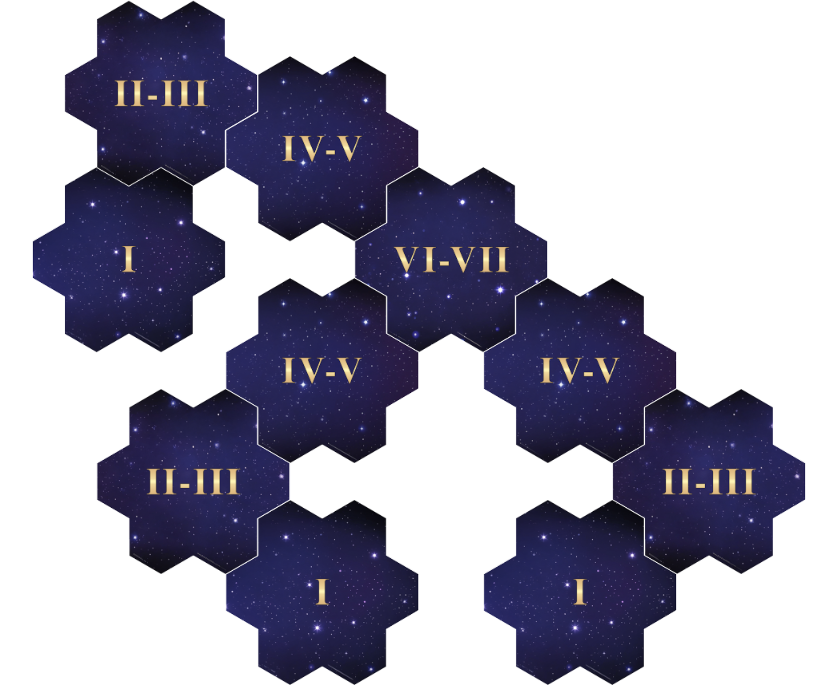
\includegraphics[scale=0.3]{\maps/stand_united_3p.png}};
  \node at (14.1, -5) {\footnotesize{\textbf{\MakeUppercase{3-PLAYER SCENARIO}}}};
  \node at (5, -5) {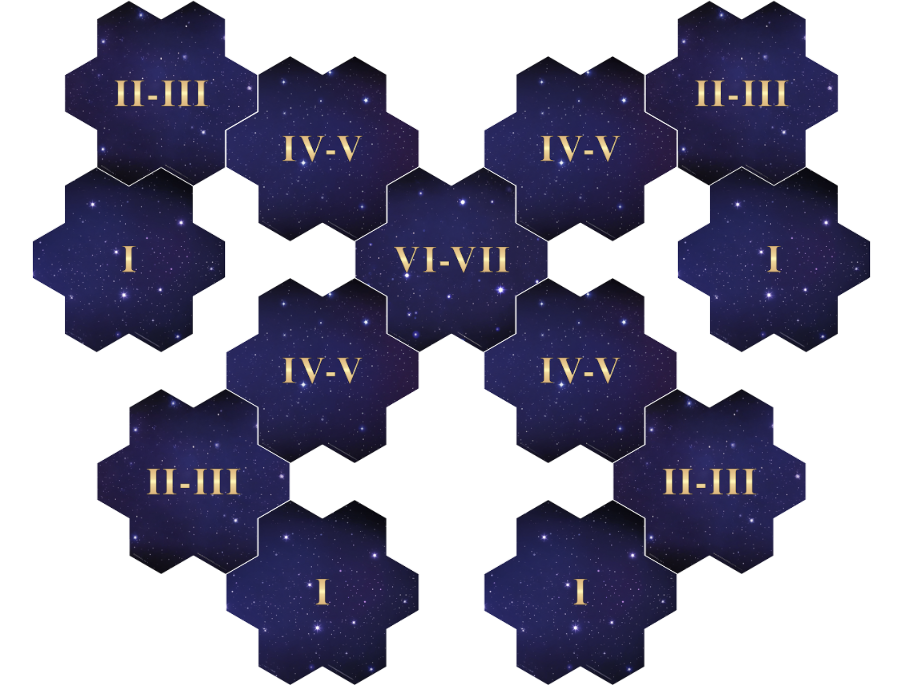
\includegraphics[scale=0.31]{\maps/stand_united_4p.png}};
  \node at (5, -10) {\footnotesize{\textbf{\MakeUppercase{4-PLAYER SCENARIO}}}};
\end{tikzpicture}

